\documentclass[journal, a4paper]{IEEEtran}

\usepackage{graphicx}   
%\usepackage{subfigure}
\usepackage{url}        
\usepackage{amsmath}  
\usepackage{hyperref}
  
% Some useful/example abbreviations for writing math
\newcommand{\argmax}{\operatornamewithlimits{argmax}}
\newcommand{\argmin}{\operatornamewithlimits{argmin}}
\newcommand{\x}{\mathbf{x}}
\newcommand{\y}{\mathbf{y}}
\newcommand{\ypred}{\mathbf{\hat y}}

\begin{document}

% Define document title, do NOT write author names
\title{An artificial intelligence in a multiplayer snake game}
\author{Anonymous Authors}
\maketitle

% Write abstract here
\begin{abstract}
Snake is a very common video game with many variations. First it has been popularized as a singleplayer game on game consoles, and more, on Nokia mobile phones. More recently it has regained attention with the release of \emph{slither.io}, a multiplayer browser game, largely inspired by the original snake game. Each player controls a snake and aims to grow in size by consuming candies. Different types of strategies can be used to this end. The objective of this project is to design an artificial intelligence in an environment which reproduces the main characteristics of \emph{slither.io}.

\end{abstract}

% Each section begins with a \section{title} command
\section{Introduction}
In this project we design an environment which looks like \emph{slither.io}, while simplyfing some features to ease the training and the design of agents. 

Regarding the environment a graphical interface is available, we reuse the interface of the project 
\footnote{http//github.com/bhairavmehta95/slitherin-gym}. We completely rebuild the backend to make it more efficient. Then we design two types of artificial intelligence. One is based on tree search methods. The other one consists in reinforcement learning algorithm.

Describe what you did. Provide access to your anonymized code\footnote{Our code is available here: \url{http://anonymouslinktoyourcode.zip}}.

Note that results should be reproducible using the technologies from the labs (i.e., Python, and selecting among Scikit-Learn, OpenAI Gym, TensorFlow, PyGame, \ldots).

Do not change the formatting (columns, margins, etc). Hint: shared tools like \texttt{http://sharelatex.com/} and \texttt{http://overleaf.com/} are great tools for collaborating on a multi-author report in latex. If you wish to use Word, base it on the IEEE template\footnote{\url{https://www.ieee.org/publications_standards/publications/conferences/2014_04_msw_a4_format.doc}} and convert to \texttt{pdf} for submission. 

\section{Background and Related Work}

Elaborate (in your own words) the background material required to understand your work. It should cover a subset of the topics touched upon in the course. You are encouraged to cite topics in lectures, e.g., structured output prediction in \cite{LectureSOP}, book chapters, e.g., Chapter 9 from \cite{Barber}, or articles from the literature, e.g., \cite{Astar,DeepMindSC2}. Basically, you should prepare the reader to understand what you are about to present in the following sections. Eq.~\eqref{eq:MAP} shows a random equation.
\begin{equation}
	\label{eq:MAP}
	% Note the example \newcommand s defined above which make it faster to write latex math
	\ypred = \argmax_{\y \in \{0,1\}} p(\y|\x)
\end{equation}

\section{The Environment}

Describe your environment, either one you adapted/borrowed from somewhere, or designed yourself. Convince the reader that it is an interesting and/or challenging environment (could it potentially have real-world use or is based on real-world data? Or simply to provide an interesting/fun/challenging problem to tackle. In particular you should outline the particular challenges it poses as a RL problem.

\section{The Agent}

The agent you designed for your environment. Justify your choice and design and explain briefly how you implemented/configured it. Naturally, if you took a ready-made environment, you should invert relatively much more effort into this section than the previous one.

\section{Results and Discussion}

This is one of the most important sections. You put your agent to the test in the environment, you show -- and most importantly -- you interpret the results.

\subsection{Performance of your Agent in your Environment}

Show plots, graphs, tables (e.g., Table~\ref{a_table}), etc. You may wish to encourage readers to reproduce results for themselves, e.g., run \texttt{runDemo.py} in our source code. Show how your agent performs well, or, if it doesn't perform well, it is better to explain why (this is a result in itself!). In any case, you \emph{must} highlight the weaknesses of your agent as well as its strengths.

\begin{table}[h]
	\caption{\label{a_table}This table is just an example.}
	\centering
	\begin{tabular}{lll}
		\hline
		\textbf{Environment config.} & \textbf{Standard SARSA} & \textbf{Our Improved Agent}  \\
		\hline
		Simulation 1        & 10             & 15 \\
		Simulation 2        & 12             & 11 \\
		\hline
	\end{tabular}
\end{table}

\subsection{Performance of your Agent in the ALife Environment}

You deploy your agent in the ALife\footnote{\url{https://github.com/jmread/alife}} environment (a random screenshot shown in Figure~\ref{a_figure}). Does it work well? Why? Why not? Justify the adaptation you think is best.

\begin{figure}[h]
	\centering
	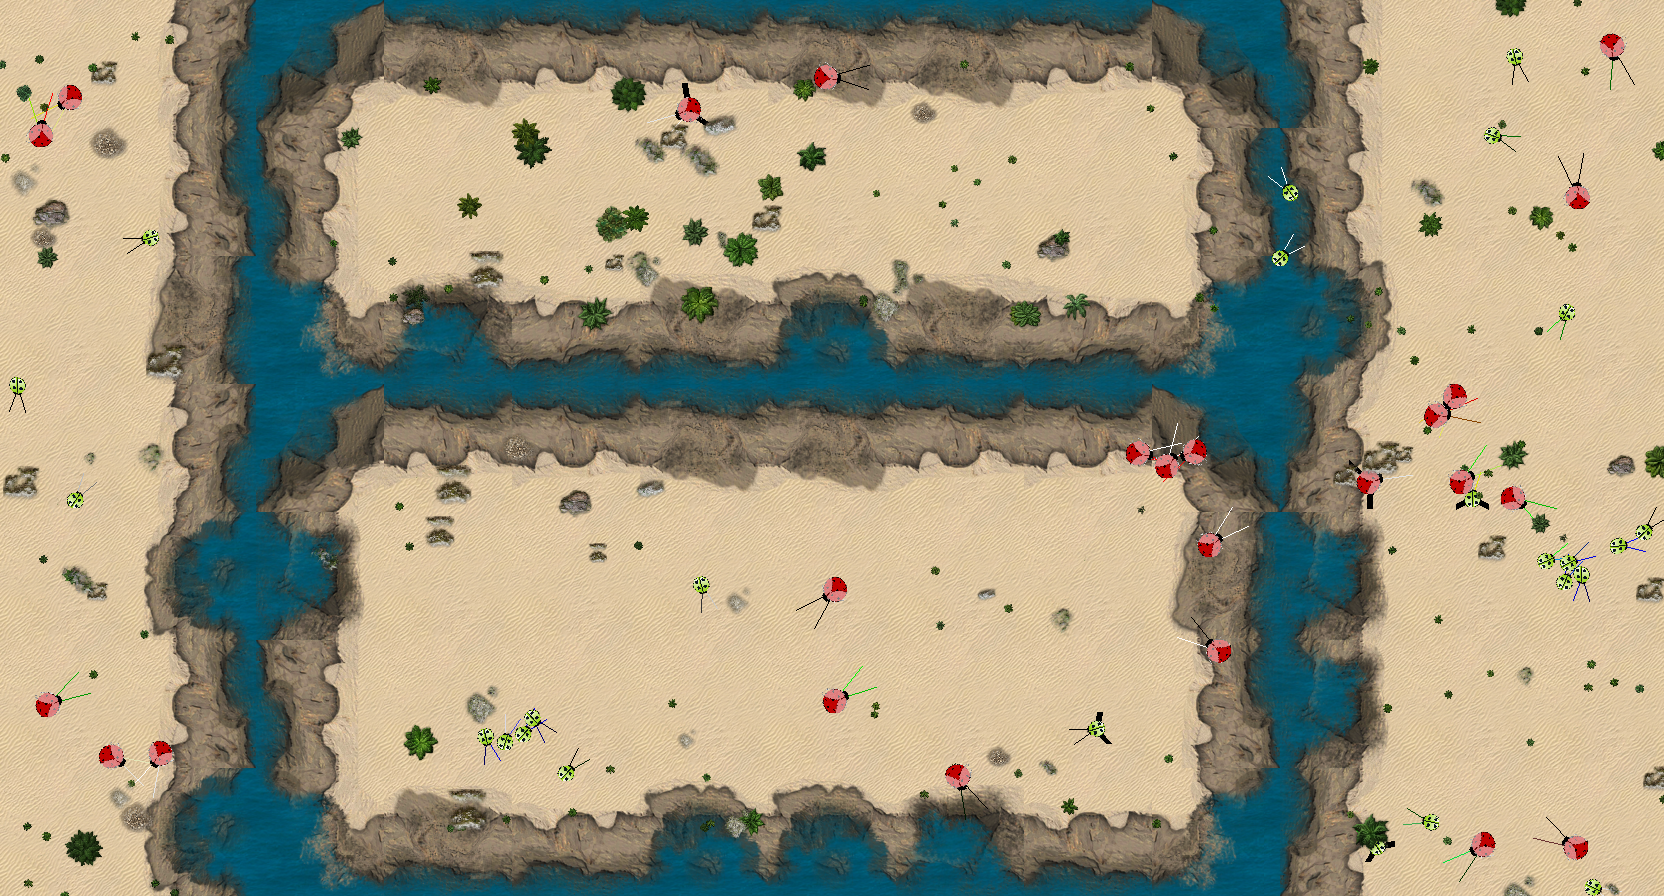
\includegraphics[width=0.8\columnwidth]{alife.png}
	\caption{\label{a_figure}An example figure}
\end{figure}


\section{Conclusion and Future Work}
	This section summarizes the paper: Your environment and agent, its strength and its weaknesses. Also remark about what would be the next steps you would take if you or someone else were to continue/extend this project. 
	Note that for the initial submission you are limited strictly to 4 pages (double column), \emph{not including references}. An extra page will be allowed for final submission (after the initial reviews). 

% The bibliography:
\begin{thebibliography}{4}

	\bibitem{Barber} % Book
	D.~Barber. Bayesian Reasoning and Machine Learning,
	{\em Cambridge University Press}, 2012.

	\bibitem{LectureSOP} % Web document
		J.~Read. Lecture III - Structured Output Prediction and Search. \textit{INF581 Advanced Topics in Artificial Intelligence}, 2018.

	\bibitem{Astar}
	D.~Mena et al. A family of admissible heuristics for A* to perform inference in probabilistic classifier chains.
	{\em Machine Learning}, vol. 106, no. 1, pp 143-169, 2017.

	\bibitem{DeepMindSC2}
	O.~Vinyals et al. StarCraft {II:} {A} New Challenge for Reinforcement Learning.
	\url{https://arxiv.org/abs/1708.04782}, 2017. 

\end{thebibliography}

% Your document ends here!
\end{document}
